\section{Two sample testing}

\begin{frame}
  \begin{center}
    {\bf Part I -- Two Sample Testing}
  \end{center}
\end{frame}

\subsection{Motivation}

\begin{frame}{Last Lecture Recap}
  In the last lecture we studied how we can use \structure{Statistical Inference} to determine the answer to questions about experimental data. For example: {\bf "are the observations produced by process B different from an expected value N?"}\bigskip

  We used the \structure{Null Hypothesis Statistical Testing} method to answer this question:
  The process of interest is modeled as a Random Variable under a normal distribution. From the sample data, we calculate a {\bf test statistic} that tells us "how surprising" that sample is under the null hypothesis.\bigskip

  Based on this information, we could answer that simple question. What about more complex situations?
\end{frame}


\begin{frame}{Comparison of two processes}
  The comparison between two different approaches is a very common situation in scientific research:\bigskip

  \begin{itemize}
    \item The efficacy of a new drug is compared against a control group;

    \item The precision of a new algorithm is compared against an old one;

    \item Two different website design proposals are compared regarding user preference;

    \item etc;
  \end{itemize}
  \bigskip

  How can we adapt the Hypothesis testing procedure studied in the last lecture to these situations?\bigskip

  The analisys of these situations involves the calculation of statistics based on data from two different samples, so we will call it {\bf two sample testing}.
\end{frame}


% \begin{frame}{Statistical Inference for Two Samples}
%   Sometimes we are interested on the comparison between two different populations, based on information from their samples. This type of analysis is frequent when we compare the effect of a technique ({\bf or treatment}) against a \emph{control group}: a placebo, a classical technique, a random search, etc;\bigskip
%
%   The statistics used in this case are actually very similar to the statistics used for the analysis of single populations; and in general the experiment design follow the same principles.\bigskip
%
%   Usual questions involve:
%   \begin{itemize}
%     \item The comparison of means;
%     \item The comparison of variances;
%     \item The comparison of proportions;
%     \item Etc;
%   \end{itemize}
% \end{frame}

\subsection{Steel Rods Example}
\begin{frame}[t]{Example: Comparing Methods for cutting steel rods}

  \begin{block}{}
  We will use the following situation to illustrate the hypothesis testing method:
  \end{block}

  \begin{columns}[T]
    \column{.2\textwidth}
    
\includegraphics[width=\textwidth]{../img/steelrods}
    \ppagenote{Steel rod image: \url{http://www.shutterstock.com/pic-73207399/}}
    \column{.8\textwidth}
    A critical aspects of manufacturing steel rods is cutting the bars with a precise length. \bigskip

    Errors when cutting the bars will cause costs for reprocessing the rods.\bigskip

    An engineer is interested in comparing the current cutting process with a new method that could potentially improve the performance of the system by reducing the cutting error.
  \end{columns}
  \bigskip
\end{frame}

\begin{frame}[t]{Comparing cutting methods}{Quiz}
  \begin{columns}[T]
    \column{.2\textwidth}
    
\includegraphics[width=\textwidth]{../img/steelrods}
    \column{.8\textwidth}
    We have two methods for cutting steel rods (old and new), and we want to find out which one has the smallest cutting error. Consider the following questions:
    {\smaller
    \begin{itemize}
      \item How do we calculate / measure the cutting error of one of the methods?
      \item What is the observation / sample necessary to estimate this value?
      \item What is the variable that measures the cutting error difference between the two methods?
      \item What is a \emph{statistical hypothesis} that represents the question of interest for this experiment?
    \end{itemize}}\bigskip

    \alert{Pause the video}! Take some time to seriously answer these questions before you continue the material!
  \end{columns}
\end{frame}

\begin{frame}[t]{Modeling the cutting process}{What is the cutting error?}
  \begin{columns}[T]
    \column{.2\textwidth}
    
\includegraphics[width=\textwidth]{../img/steelrods}
    \column{.8\textwidth}
    Let's look at the first two questions:
    \begin{block}{}
    {\smaller
    \begin{itemize}
      \item How do we calculate / measure the cutting error of one of the methods?
      \item What is the observation / sample necessary to estimate this value?
    \end{itemize}}
    \end{block}\bigskip

    Let's consider a cutting error to be the difference between the length of a rod $i$ and the target length $l$: ($|x_i - l|$). \bigskip

    Assuming that the cutting error is a property of the method, we can estimate the \structure{mean cutting error} using a sample $X$ of $n$ rods:
    \begin{equation*}
      \hat\mu_e \text{ estimated by } e_X = \frac{\sum{|x_i - l|}}{n}
    \end{equation*}
  \end{columns}
\end{frame}

\begin{frame}[t]{Modeling the cutting process}{Cutting Error and Hypothesis}
  \begin{columns}[T]
    \column{.2\textwidth}
    
\includegraphics[width=\textwidth]{../img/steelrods}
    \column{.8\textwidth}
    \begin{equation*}
      \hat\mu_e \text{ estimated by } e_X = \frac{\sum{|x_i - l|}}{n}
    \end{equation*}

    Using $e_X$ as an estimate of the cutting error, it is possible to to perform statistical inference about \structure{one of the methods}. For example:\bigskip

    \begin{itemize}
      \item Is the error of method $Y$ equal or under a required value $r$?
      \item $H_0: e_Y \leq r$
      \item $H_1: e_Y \geq r$
    \end{itemize}\bigskip

    We can use the technique from the last lecture to solve this problem. But if we want to compare two methods: $Y_1$ and $Y_2$, what do we do?
  \end{columns}
\end{frame}

\begin{frame}[t]{Modeling the cutting process}{Comparing Errors}
  \begin{columns}[T]
    \column{.2\textwidth}
    
\includegraphics[width=\textwidth]{../img/steelrods}
    \column{.8\textwidth}
    \begin{block}{}
    {\smaller
    \begin{itemize}
      \item What is the variable that measures the cutting error difference between the two methods?
      \item What is a \emph{statistical hypothesis} that represents the question of interest for this experiment?
    \end{itemize}}
    \end{block}
    Let's consider these two questions. Remember that the error from each method is modeled as a random variable following a normal distribution.
    \begin{center}
      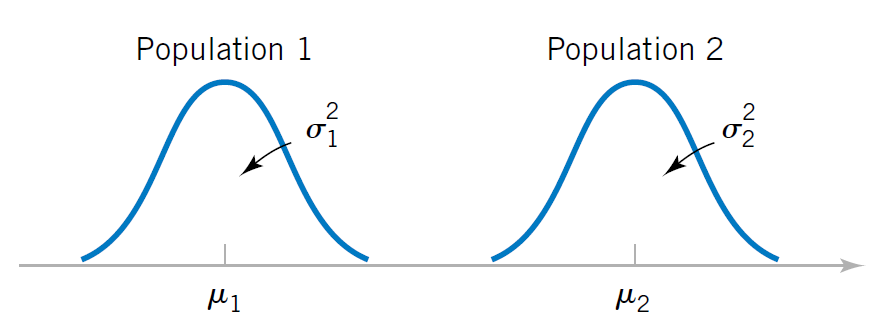
\includegraphics[width=.5\textwidth]{../img/two_population_model}
      \ppagenote{Two models image from D.C. Montgomery "Applied Statistics and Probability for Engineers", Wiley 2003}
    \end{center}
  \end{columns}
\end{frame}

\begin{frame}[t]{Modeling the cutting process}{Comparing Errors}
    \begin{center}
      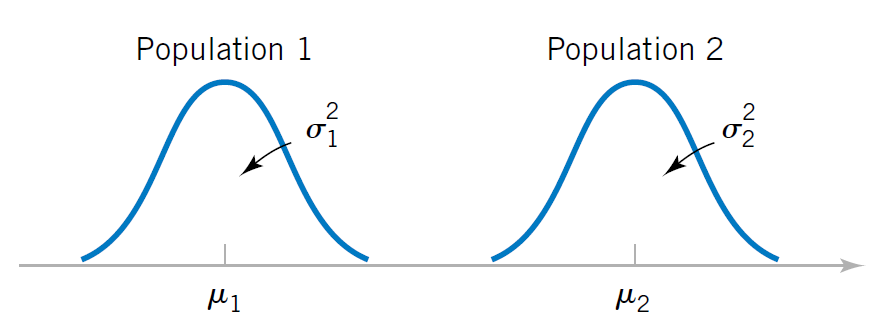
\includegraphics[width=.4\textwidth]{../img/two_population_model}
      \ppagenote{Two models image from D.C. Montgomery "Applied Statistics and Probability for Engineers", Wiley 2003}
    \end{center}

    The sum of two normal variables also follow a normal distribution. So, we can describe the difference between the cutting errors as the random variable $e_{\text{diff}}  = (e_{\text{old}} - e_{\text{new}})$.\bigskip

    Because $e_{\text{diff}}$ also follows a normal distribution, we can use the null hypothesis method to test the difference of the two methods:
    \begin{itemize}
      \item $H_0: e_{\text{diff}} = 0$
      \item $H_1: e_{\text{diff}} \neq 0$
    \end{itemize}
\end{frame}

\subsection{General Statistical Model}
\begin{frame}{A General Model for Comparing two Samples}
  Using the ideas from the previous example, let's describe a general statistical model to use when we want to test if two methods are quantitatively different.\bigskip

  Consider that we measure some observed value ($y$) taken from one of several methods ($i = 1, 2,\ldots$), we understand that the value comes from some distribution with mean $\mu_i$, at it will also have an error ($\epsilon$) away from that mean, which is different for each observation. So we describe the $j$-th observation taken from the $i$-th method as

  \begin{equation*}
    y_{ij} = \mu_i + \epsilon_{ij}\begin{cases}i=1,2\\j=1,\ldots,n_i\end{cases}
  \end{equation*}
\end{frame}

\begin{frame}{Statistical Models}{Two population Model}
  \begin{equation*}
    y_{ij} = \mu_i + \epsilon_{ij}\begin{cases}i=1,2\\j=1,\ldots,n_i\end{cases}
  \end{equation*}\medskip

  Under this model for the observed variable ($y_{ij}$), we assume that the residuals $\epsilon_{ij}$ are independent and follow $\mathcal{N}\left(0,\sigma_i^2\right)$. Under these assumptions, the populations of the two samples look like this:

  \begin{center}
    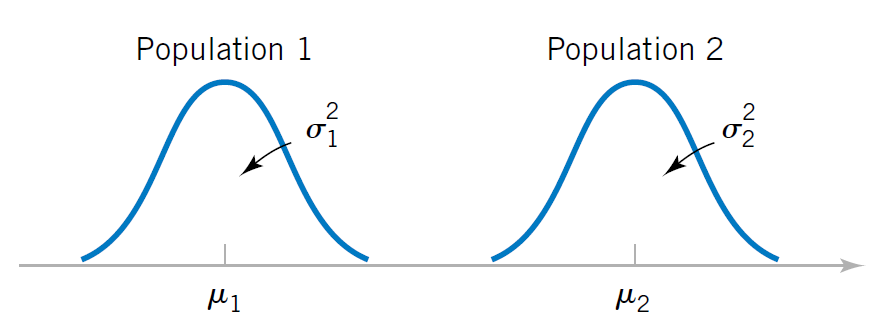
\includegraphics[width=.5\textwidth]{../img/two_population_model}
  \end{center}
\end{frame}

\begin{frame}{Comparison of two means}{Null and Alternate Hypotheses}

What should be the observed variable $y$? The goal of this experiment is to measure if the new method produces steel rods closer to the nominal value. In this case, a possible response variable would be the \structure{absolute error}, e.g., $y = |\ell - \ell_{nominal}|$.\bigskip

Keeping in mind our statistical model, we can build the hypothesis around the \structure{mean} of the absolute error ($\mu_i$). In that case, we can state the null and alternate hypotheses as:
\begin{equation*}
\begin{cases}
H_0: \mu_1 - \mu_2 = 0\\
H_1: \mu_1 - \mu_2 < 0
\end{cases}\ \ \ \mbox{\textbf{or, equivalently, }}\ \ \ \ \ \ \begin{cases}
H_0: \mu_1 = \mu_2\\
H_1: \mu_1 < \mu_2
\end{cases}
\end{equation*}
\medskip
\end{frame}



\begin{frame}{Comparison of two means}{Calculating the statistic}

  Lets assume (for the moment) that the variance of the process is unknown but similar for both systems. Since it is unknown, we have to estimate the variance from the sample data. As assume $\sigma^2_1\approx\sigma^2_2$, we can use the pooled variance estimator:

\begin{equation*}
s_p^2 = \frac{\left(n_1-1\right)s_1^2+\left(n_2-1\right)s_2^2}{n_1+n_2-2}
\end{equation*}
\bigskip

Based on this estimator and the stated assumptions, we calculate the T statistic:
\begin{equation*}
T = \frac{\left(\bar{y_1} - \bar{y_2}\right) - \left(\mu_1 - \mu_2\right)}{s_p\sqrt{\frac{1}{n_1} + \frac{1}{n_2}}}\sim t^{\left(n_1+n_2-2\right)}
\end{equation*}
\end{frame}

\subsection{Calculation of the Statistic}

\begin{frame}
{Back to the Steel Rods Example}
{Calculation of the Rejection threshold}

If we recall our working hypotheses for the steel rod example:

\begin{equation*}
\begin{cases}
H_0: \mu_1 - \mu_2 = 0\\
H_1: \mu_1 - \mu_2 < 0
\end{cases}
\end{equation*}

\noindent we have that, \underline{under $H_0$}:

\begin{equation*}
t_0 = \frac{\left(\bar{y_1} - \bar{y_2}\right) - \cancelto{0}{\left(\mu_1 - \mu_2\right)}}{s_p\sqrt{\frac{1}{n_1} + \frac{1}{n_2}}} = \frac{\left(\bar{y_1} - \bar{y_2}\right)}{s_p\sqrt{\frac{1}{n_1} + \frac{1}{n_2}}}\sim t^{\left(n_1+n_2-2\right)}
\end{equation*}

We'll reject $H_0$ at the $(1-\alpha)$ confidence level if $t_0\leq t^{(n_1+n_2-2)}_{\alpha/2}$
\end{frame}

\begin{frame}
{Back to the Steel Rods Example}
{Statistic Test Parameters}

  Remember that we need to decide \structure{three parameters} that will specify the statistical test:

  \begin{itemize}
    \item {\bf Significance level}: The probability of a {\bf Type I error}. Let's assume that the desired significance level is $\alpha = 0.05$.\bigskip

    \item {\bf Power}: The probability of a {\bf Type II Error}. Let's assume that the desired sensitivity is $1 - \beta = 0.8$.\bigskip

    \item {\bf Meaningful difference}: What is the minimum difference between the two methods that we are interested in detecting? Let's assume $15cm$.
  \end{itemize}\bigskip

The values for these variables depend on the needs of the specific experiment and/or application.

\end{frame}

%%%%%%%%%%%%%%%%%%%%%%%%%%%%%%%%%%%

\begin{frame}[fragile]{Calculating the Statistic}
Computationally, we can perform the t-test for comparing the means of two independent populations by:
\bigskip
{\smaller
\begin{verbatim}
> y <- read.table("steelrods.csv", header = TRUE)
> t.test(y$Length.error ~ y$Process, alternative = "less",
+        mu          = 0, var.equal   = TRUE, conf.level  = 0.95)

data:  y$Length.error by y$Process
t = -14.312, df = 32, p-value = 9.244e-16
alternative hypothesis: true difference in means is less than 0
95 percent confidence interval:
      -Inf -7.156884
sample estimates:
mean in group new mean in group old
         7.782353         15.900000
\end{verbatim}}
\end{frame}

%=====

\begin{frame}[fragile]{Comparison of two means}{Testing the assumptions}


\begin{columns}[T]
  \column{0.7\textwidth}

  The assumptions of the test must be verified. In this particular case:


  {\smaller
\begin{itemize}
  \item \alert{Normality};
  \item Equality of variances;
  \item Independence.
\end{itemize}

{\smaller
\begin{verbatim}
> qqPlot(y$Length.error, groups = y$Process,
        cex = 1.5, pch = 16,  las = 1,
        layout = c(2, 1))
> shapiro.test(y$Length.error[y$Process == "new"])
# W = 0.92269, p-value = 0.164
> shapiro.test(y$Length.error[y$Process == "old"])
# W = 0.94971, p-value = 0.4519
\end{verbatim}}}

{\bf Reminder:} the t-test is quite robust to mild to moderate violations of the normality of the residuals / groups.
\column{.3\textwidth}
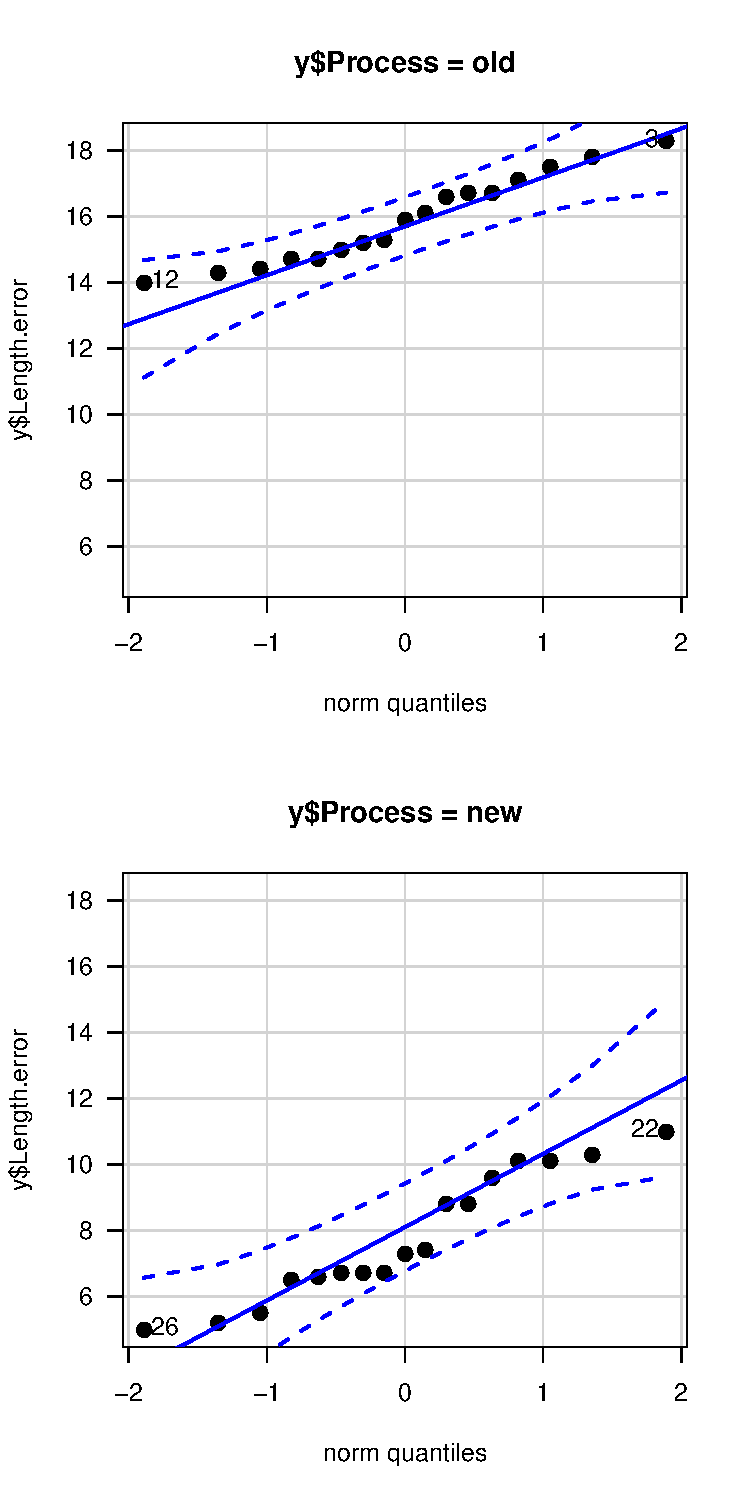
\includegraphics[width=.7\textwidth]{../img/steelrodsqq.pdf}
\end{columns}
\end{frame}

\begin{frame}[fragile]{Comparison of two means}{Testing the assumptions}
The assumptions of the test must be verified. In this particular case:

\begin{columns}[T]
  \column{.7\textwidth}
  {\smaller
    \begin{itemize}
      \item Normality;
      \item \alert{Equality of variances};
      \item Independence;
    \end{itemize}
    {\smaller
\begin{verbatim}
> fligner.test(Length.error ~ Process, data = y)
# Fligner-Killeen:med chi-squared = 1.6837,
# df = 1, p-value = 0.1944

> residuals <- tapply(X = y$Length.error,
               INDEX = y$Process,
               FUN   = function(x){x - mean(x)})

> stripchart(x        = residuals, vertical = TRUE,
             pch      = 16, cex = 1.5, las = 1,
             xlab     = "mean",
             ylab     = "residuals")
\end{verbatim}}}
\column{.3\textwidth}
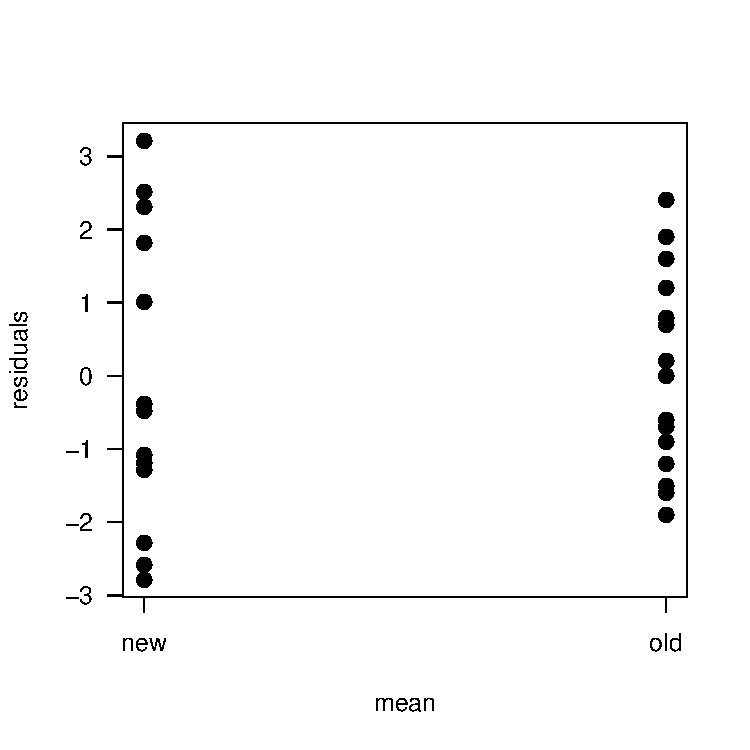
\includegraphics[width=\textwidth]{../img/steelrodsvar.pdf}
\end{columns}
\end{frame}

\begin{frame}
{Comparison of two means}
{Testing the assumptions}
The assumptions of the test must be verified. In this particular case:

{\smaller
\begin{itemize}
  \item Normality;
  \item Equality of variances;
  \item \alert{Independence};
\end{itemize}}
\bigskip

As mentioned in the last class, there is no general test for the independence assumption, and it has to be guaranteed in the design phase.
\bigskip

One can at most test for serial autocorrelation in the residuals using Durbin-Watson's test, but this test is absolutely dependent on the ordering of the observations - very useful to detect ordering-related trends in the residuals, but not much more than that.
\end{frame}

\begin{frame}{Comparison of two means}{Unequal variances}
Suppose now a more general case, in which the variances of the two populations are unknown and cannot be assumed equal.
\bigskip

For this cases, a modification on the t-test called \textit{Welch's t test} is usually employed. The Welch statistic can be calculated as:
\begin{equation*}
  t^*_0 = \frac{\bar{y_1} - \bar{y_2}}{\sqrt{\frac{s_1^2}{n_1} + \frac{s_2^2}{n_2}}}
\end{equation*}
\bigskip

Under the null hypothesis $t^*_0$  is distributed approximately as a $t^{(\nu)}$ distribution, with:
\begin{equation*}
\nu = \frac{\left(\frac{s_1^2}{n_1} + \frac{s_2^2}{n_2}\right)^2}{\frac{\left(s_1^2/n_1\right)^2}{n_1-1} + \frac{\left(s_2^2/n_2\right)^2}{n_2-1}}
\end{equation*}
\end{frame}



\begin{frame}[fragile]{Comparison of two means}{Unequal variances}
Let's illustrate the calculation of a comparison test with unequal variances in R. We will use the same data as before.\footnote{Note that this would not have been necessary, since we already checked the "equal variances" assumption.}
\bigskip

{\smaller{\smaller
\begin{verbatim}
> t.test(y$Length.error ~ y$Process, alternative = "two.sided",
+        mu = 0,
+        var.equal = FALSE,            %% <- We only change this.
+        conf.level = 0.95))
Welch Two Sample t-test
data:  Length.error by Process
t = -14.312, df = 28.386, p-value = 1.645e-14
alternative hypothesis: true difference in means is not equal to 0
95 percent confidence interval:
-0.09278780 -0.06956515
sample estimates:
mean in group new mean in group old
      0.07782353        0.15900000
\end{verbatim}}}
\end{frame}

%
% \begin{ftst}
% {Comparison of two means}
% {Unequal variances}
% The two-sample Welch t-test for considering unequal variances is usually the first test of choice, since it drops one (often inconvenient) assumption, at a very small cost in terms of power.
% \vone
% Calculating sample sizes for the general case (unequal variances, unequal sample sizes) is not particularly difficult, and can be done for either a \textit{balanced} case (i.e., $n_1 = n_2 = n$) or an optimal, \textit{unbalanced} case (in which $n_1 \neq n_2$).
% \vone
% For the unbalanced case, it is not particularly difficult to prove that the optimal allocation of observation is to keep:
% $$\frac{n_1}{n_2} = \frac{\sigma_1}{\sigma_2}$$.
%
% (if a good estimate of the ratio of variances is available, of course).
% \end{ftst}
%=====

\begin{frame}{Comparison of two means}{Summary}

  To compare an estimator from samples of two populations that follow a normal distribution, we set our statistic and the corresponding hypotheses to be the difference of the target variables.\bigskip

  This technique for comparison testing is simple and extremely versatile.\bigskip

  Of course, there are cases where this approach does not apply. Next we will see a relatively common case where using the difference of the target variables would lead to a wrong inferential result.
\end{frame}
